\documentclass[12pt]{exam}
\usepackage[utf8]{inputenc}

\usepackage{graphicx}
\usepackage{makecell}
\usepackage{minibox}
\usepackage{multirow}
\usepackage{lastpage}
\usepackage{amsmath}
\usepackage[margin=0.5in]{geometry}
\usepackage{amssymb}
\usepackage{xcolor}
\usepackage{datetime}
\usepackage{amsmath}
\usepackage{mathtools}


\pagestyle{headandfoot}

\newdateformat{monthyeardate}{%
  \monthname[\THEMONTH], \THEYEAR}
%\newdateformat{\monthyeardate}{\monthname[\THEMONTH], \THEYEAR}




\newcommand{\paper}[5]{
    \setcounter{page}{1}
    
    \begin{minipage}{\textwidth}
    \Large{\textbf{Tougaloo College}}\\
    %\vspace{0.1in}\\  
   % Bachelor of the Science of Engineering \\
    %Academic Year #4\\
    %\vspace{0.1in}\\
    \textbf{#2}\\
    \textbf{#5 - #3}\\
    \end{minipage}
    \hfill
   % \begin{minipage}{3in}
      %  \centering
      %  \includegraphics[scale=0.23]{logo.jpg}
    %\end{minipage}\\
    %\hfill
   % \vspace{0.1in}\\
        \begin{minipage}{6in}
            \textbf{\hspace{0.25in}Due Date : #1}
        \end{minipage}
    
    \vspace{0.1in}
    \rule[1ex]{\textwidth}{2pt}
    }



\extrafootheight{.5in}
\cfoot{Page ~\thepage ~of ~\numpages}


\printanswers


\marginpointname{ \points}
\pointsinrightmargin
\pointpoints{ Point}{ Points}
\setlength{\rightpointsmargin}{3cm}
\pointsdroppedatright
\addpoints
%\qformat{\textbf{Question \thequestion} \hfill}

%%%%%%%%%%%%%%%%%%%%%%%%%%%%%%%%%%%%%%%%%%%%%%%%%%%%%%%%
%%%%%%%%%%%%%%%%%%%%%%%%%%%%%%%%%%%%%%%%%%%%%%%%%%%%%%%%


\begin{document}
%\paper{duration}{Course}{Semester}{academic year}{Examination}
\paper{03/28/2025}{MAT426 - Advanced Calculus}{Spring, 2025}{}{Howework 05}

\section*{Basic Topology - Exercises}
\begin{questions}



\question[] (Problem 9) Let \(E^0\) denote the set of all interior points of s set \(E\). 

\begin{parts}
    \part[3] Prove that \(E^0\) is always an open set.
    \begin{solution}
        Use definition 2.18(e) and theorem 2.19.
    \end{solution}
    \droppoints
    \part[3] Prove that \(E\) is open if and only if \(E^0=E\).
    
    \droppoints
    \part[3] If \(G \subset E\) and \(G\) is open, prove that \(G \subset E^0\).
    \droppoints
    \part[3] Prove that the complement of \(E^0\) is the closure of the complement of \(E\).
    \droppoints
    \part[4] Do \(E\) and \(\overline{E}\) always have the same interior points? 
    \droppoints
    \part[4] Do \(E\) and \(E^0\) always have the same closure points? 
    \droppoints
\end{parts}


\droptotalpoints

%\question[20] (Problem 36) Let \(G\) be a group and let \(a \in G\). Prove that \(C(a) = C(a^{-1}).\)

\question[] (Problem 14) Give an example of an open cover of the segment \((0,1)\) which has no finite sub cover. 

\begin{solution}

    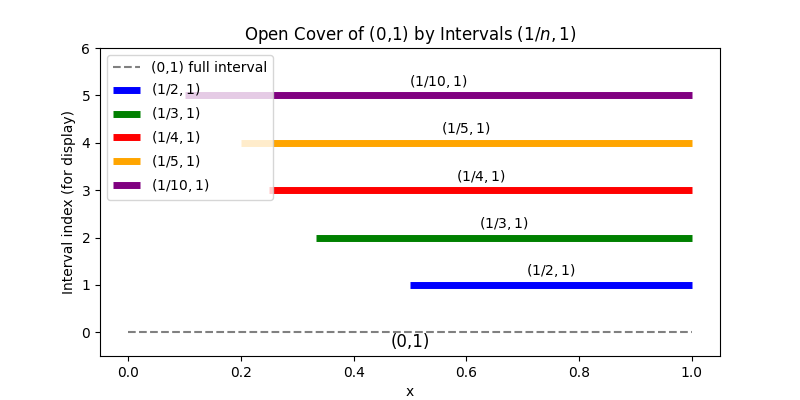
\includegraphics[scale=0.5]{figures/Figure_1.png}


    The collection of open intervals \[\mathcal{U} = \left\{\left(\dfrac{1}{n},1\right)|n \in \mathbb{N}, n \geq 2\right\}\]
is an open cover of \((0,1)\) because for any \(x \in (0,1)\), there exists a sufficiently large \(n\) such that \(x \in (1/n,1)\). However, it does not have a finite subcover; if it did, some points near 0 would be missed. 
\end{solution}

\question[] (Problem 16) Regard \(\mathbb{Q}\), the set of all rational numbers, as a metric space, with \(d(p,q)=|p-q|\). Let \(E\) be the set of all \(p\in \mathbb{Q}\) such that \(2<p^2<3\). Show that \(E\) is closed and bounded in \(\mathbb{Q}\), but that \(E\) is not compact. Is \(E\) open in \(\mathbb{Q}\)? 

\begin{solution}
    \[E = \{p \in \mathbb{Q}| 2 < p^2<3\} = \{\mathbb{Q} \cap \{(-\sqrt{3}, -\sqrt{2}) \cup (\sqrt{2}, \sqrt{3})\}\}\] 
    Since \(|p|< \sqrt{3}\), \(E\) is bounded. \\
For any sequence in \(E\), converge within \(E\) since the \(\pm \sqrt{2}, \pm \sqrt{3}\) are irrational. 

\textcolor{red}{Complete!}

\end{solution}







%%%%%%%%%%%%%%%%%%%%%%%%%%%%%%%%%%%%%%%%%%%%%%%%%%%%%%%%%
%%%%%%%%%%%%%%%%%%%%%%%%%%%%%%%%%%%%%%%%%%%%%%%%%%%%%%%%%
\end{questions}
\end{document}


